\documentclass[letterpaper,10pt]{article}

\usepackage{titling}
\usepackage{listings}
\usepackage{url}
\usepackage{setspace}
\usepackage{subfig}
\usepackage{sectsty}
\usepackage{pdfpages}
\usepackage{colortbl}
\usepackage{multirow}
\usepackage{multicol}
\usepackage{relsize}
\usepackage{amsmath}
\usepackage{wasysym}
\usepackage{fancyvrb}
\usepackage{amssymb}
\usepackage{ifsym}
\usepackage{amsmath,amssymb,amsthm,graphicx,xspace}
\usepackage[titlenotnumbered,noend,noline]{algorithm2e}
\usepackage[compact]{titlesec}
\usepackage{XCharter}
\usepackage[T1]{fontenc}
\usepackage{tikz}
\usetikzlibrary{arrows,automata,shapes,trees,matrix,chains,scopes,positioning,calc}
\tikzstyle{block} = [rectangle, draw, fill=blue!20, 
    text width=2.5em, text centered, rounded corners, minimum height=2em]
\tikzstyle{bw} = [rectangle, draw, fill=blue!20, 
    text width=4em, text centered, rounded corners, minimum height=2em]

\definecolor{namerow}{cmyk}{.40,.40,.40,.40}
\definecolor{namecol}{cmyk}{.40,.40,.40,.40}

\let\LaTeXtitle\title
\renewcommand{\title}[1]{\LaTeXtitle{\textsf{#1}}}


\newcommand{\handout}[5]{
  \noindent
  \begin{center}
  \framebox{
    \vbox{
      \hbox to 5.78in { {\bf ECE356: Database Systems } \hfill #2 }
      \vspace{4mm}
      \hbox to 5.78in { {\Large \hfill #4  \hfill} }
      \vspace{2mm}
      \hbox to 5.78in { {\em #3 \hfill} }
    }
  }
  \end{center}
  \vspace*{4mm}
}

\newcommand{\lecture}[3]{\handout{#1}{#2}{#3}{Lecture #1}}
\newcommand{\tuple}[1]{\ensuremath{\left\langle #1 \right\rangle}\xspace}

\addtolength{\oddsidemargin}{-1.000in}
\addtolength{\evensidemargin}{-0.500in}
\addtolength{\textwidth}{2.0in}
\addtolength{\topmargin}{-1.000in}
\addtolength{\textheight}{1.75in}
\addtolength{\parskip}{\baselineskip}
\setlength{\parindent}{0in}
\renewcommand{\baselinestretch}{1.5}
\newcommand{\term}{Winter 2018}

\singlespace


\begin{document}

\lecture{ 19 --- Query Optimization }{\term}{Jeff Zarnett}

\section*{Query Optimization}

Given an understanding of the various rules, there are now some clear ways we can transform an input query to determine which of the equivalent representations will have the lowest cost of execution. Combining that with what we have already seen when it comes to join operations, it is fair to say that the query optimizer is likely to focus first on join relations since that is potentially the biggest area in which we can make some gains.

Suppose our query involves a selection and a join: we want to select the employee number, salary, and address for an employee with an ID of 385. Suppose number and salary are in the employee table with 300 entries, and the address information is in another table with 12000 entries. We have a join query, and if we do this badly, we will compute the join of employees and addresses, producing some 300 results, and then we need to do a selection and a projection on that intermediate relation. If done efficiently, we will do the selection and projection first, meaning the join needs to match exactly one tuple of employees rather than all 300. 

The query optimizer should systematically generate equivalent expressions, but since performing all possible transformations and then evaluating each option may itself take non-trivial time, it is likely that the optimizer does not consider every possibility and will take some ``shortcuts'' rather than brute force this. One technique that helps on top of that is to re-use common subexpressions to reduce the amount of space used by representing the expressions during evaluation~\cite{dsc}.

\subsection*{Estimating Statistics}

For all the discussion about how it might make sense to swap this or change that or do this rather than that, we have not yet really talked about how the system may guess about how many results are going to be returned. In the previous example I used exact numbers, 300... 1... 12000... etc., but for the database server to get those it can either look them up, or it can guess about them. As mentioned earlier, sometimes certain numbers, like the number of tuples in a relation, are easily available by looking at metadata. If we want to know, however, how many employees have a salary between \$40~000 and \$50~000, the only way to be sure\footnote{Other than nuking it from orbit...} is to actually do the query, and we most certainly do not want to do the query when estimating the cost, since at that point we might as well not bother optimizing at all.

If we cannot measure, then, well, we need to guess. Our guesses are, however, not wild, but instead educated. Estimates are based on assumptions, and those assumptions are very often wrong. That is okay. We do not need to be perfect. All we need is to be better than not optimizing. And even if we pick the second or third or fifth best option, that is acceptable as long as we are close to the best option.

There are five major areas where costs for actually performing a query accumulates. We have, for simplicity, acted as if accessing disk storage is much larger than any other costs to the point where it dominates all other factors. That is not quite accurate, and modern query optimizers are capable of taking more things into consideration. The list from~\cite{fds} below is more complete:

\begin{enumerate}
	\item \textbf{Disk I/O}: the previously-discussed costs of seeking and data transfer to get data from the disk or other secondary storage.
	\item \textbf{Disk Additional Storage}: the costs, if any, of storing intermediate relations on disk during processing of the query.
	\item \textbf{Computation}: The CPU usage that will be required to do the operations including sorting, merging, and arithmetic operations.
	\item \textbf{Memory}: The memory usage for the buffers necessary to do the desired operations.
	\item \textbf{Communication}: The cost of sending the results back to the requester, or in  a distributed database, the cost of transferring data between the different nodes.
\end{enumerate}

We will generally proceed on the basis that disk I/O is the largest cost and outweighs everything else. That may not be true in a particular use case (e.g., the database server has tons of RAM and a lot of data can be kept in memory). The principles of assessing cost and choosing a strategy still apply, even if we are optimizing faster queries or constrained by CPU instead of disk.

\paragraph{Metadata.} As previously mentioned, there is some metadata stored in the database that we could look at to find out some data that we know has some high accuracy. Some items that might be in the metadata, from~\cite{dsc} and ~\cite{fds}:

\begin{itemize}
	\item $n_{r}$: the number of tuples in a relation $r$ 
	\item $b_{r}$: The number of blocks containing a relation $r$ 
	\item $l_{r}$: the size in bytes of relation $r$
	\item $f_{r}$: the number of tuples of $r$ that fit into one block
	\item $V(A, r)$: the number of distinct values in $r$ of attribute $A$
	\item $h_{r, i}$: the height of an index $i$ defined on relation $r$
\end{itemize}

Some of these values can be computed, notably $l_{r}$ is the number of blocks times the size of a block, and $f_{r}$ is the number of tuples divided by the number of blocks. The value of $V(A, r)$ may or may not be maintained for all attributes, or for groups if that is so desired. If it is on a key field, every value is unique, so we know it is the same as the number of tuples for that field. There can also be metadata about index information as well... which might make it metametadata? 

There are obviously tradeoffs when it comes to maintaining metadata. The more often it is updated, the more effort is spent updating it. If every insertion or update or deletion resulted in an update, that may mean a nontrivial amount of time is spent updating this data. If we only do periodic updates, it likely means that the statistic data will be outdated when we go to retrieve it for use in a query optimization context. Perhaps some amount of balance is necessary: updates can be done during times of lower system load with some maximum limit for how long an update can wait before it gets enough priority. This is, in some small way, a callback to scheduling algorithms you have surely learned about in an OS class. 

A database may also be interested in keeping some statistical information in a histogram. The values are divided into ranges and we have some idea of how many tuples are in those ranges. You have almost certainly seen a histogram before in something like a population pyramid diagram. An example from~\cite{dsc}:

\begin{center}
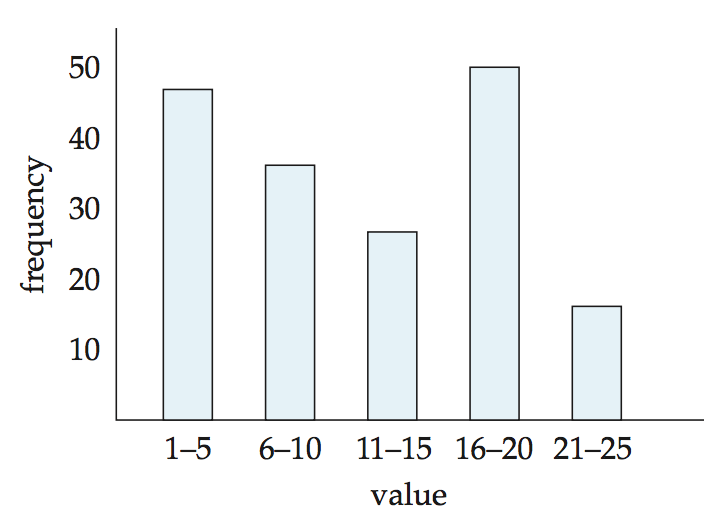
\includegraphics[width=0.4\textwidth]{images/histogram}
\end{center}

That should also tell you that they do not necessarily have an even distribution. A histogram does not take up a lot of space and it can help us to figure out certain problems: if we have a histogram of salaries and the largest bucket is 100~000+ and there are 10 people in this category, and there is a query asking how many employees have a salary greater than or equal to \$100~000 we will know at least that the number of tuples to be returned is 10. Nice.

The above numbers are exact values which we can know and, hopefully, trust although they could be slightly out of date depending on when exactly metadata updates are performed. The more exact values we have, the better our guesses. But things start to get interesting when, in the previous example, we ask something that does not have a category, such as how many people have a salary larger than \$150~000, where there isn't an obvious answer found in the metadata?

As in the previous discussion of costs, we expect select operations and join operations to be the important ones since they are the ones we will do the most of (probably). Our strategies again come from~\cite{dsc}: 

\subsection*{Estimating Selection Size}

We will start with select operations.


\paragraph{Single Equality Predicate.} The base case to consider is a single predicate in a selection with an equality condition (e.g., province = ``ON''). The estimate depends on what we know about the attribute $A$ referenced in the selection. If it is a key field, and therefore unique, we know the select will return 1 result. Unless, of course, it is not found and we will get zero results; but usually we do not expect that sort of result. 

If values are evenly distributed, then we can expect that $n_{r}/V(A, r)$ tuples should be returned. If there are ten possible values and everything is approximately evenly distributed then a select is expected to produce approximately 10\% of the tuples as its result. The uniform distribution may not be accurate, but if it is a reasonable approximation of the data, it is simple and fast. If a histogram is available, we can look in the range that contains that search value and guess based on the frequency count for that range instead.

\paragraph{Single Comparison Predicate.} 
The next case is when we have a comparison like the salary greater than or equal to \$150~000 then we can, using the known maximum and minimum values of this attribute, take a guess. If the requested value $v$ is less than the minimum, we expect no rows returned; if the requested value is greater than the max also zero. Otherwise, the formula to estimate, where $m$ is the minimum value and $M$ is the maximum value: $n_{r} \times \dfrac{v - m}{M - m}$

Of course, if a histogram is available, we would prefer to use that. 

\paragraph{Complex Predicates.}
For conjunction as well as disjunction, we will use a new symbol, $s$, which represents the selectivity of the a particular selection: how likely it is that a particular tuple matches a condition. The probability that a tuple satisfies $\theta_{i}$ is $s_{i}/n_{r}$.

For conjunctive selection, we want the probability that a certain tuple meets all of the criteria. So the formula to estimate is:

$n_{r} \times \dfrac{s_{1} \times s_{2}... \times s_{k}}{(n_{r})^{k}}$.

For disjunctive selection it is the probability of matching an one of those conditions. The calculation will be simplified by trying to compute 1 minus the probability it satisfies none of the conditions: 

$1 - (1 - \dfrac{s_{1}}{n_{r}}) \times (1 - \dfrac{s_{2}}{n_{r}}) \times ... \times (1 - \dfrac{s_{k}}{n_{r}})$

Negation is pretty simple: if we have a predicate $\neg\theta$ then the number of tuples likely to meet that is the number of tuples in the relation subtract those that do match $\theta$.

\subsection*{Estimating Join Size}

If we are computing a join where the relations have no attributes in common, then the ``join'' is really the cartesian product and the number of tuples in the output will be the number of tuples in $r_{1}$ multiplied by the number of tuples in $r_{2}$. That's a lot.

If the intersection of $r_{1}$ and $r_{2}$ is a key (unique value) for $r_{1}$ then we know that a tuple in $r_{2}$ can match with at most one in $r_{1}$ so the maximum number of tuples that could occur is the number of tuples in $r_{2}$. If the intersection is also defined as a foreign key on $r_{2}$ then it is exactly the number of tuples in $r_{2}$. This also applies symmetrically (so you can swap $r_{1}$ and $r_{2}$ in the previous statements).

The difficult case occurs if the intersection of two relations is not a key in either of those two relations. In that case, looking at the attributes in the relation, which we will call $A$, then the number of tuples in the join relation are:

$\dfrac{n_{r_{2}}}{ V(A, r_{2})} $. 

In other words, the average number of values in $r_{2}$ that have a given value of $A$. Since we expect that they match with $r_{1}$ then we estimate that there will be:

$\dfrac{n_{r_{1}} \times n_{r_{2}}}{ V(A, r_{2})} $. 

Now wait, you might say, because the denominator here depends only on $r_{2}$, and if you switched the positions of $r_{1}$ and $r_{2}$ we could get a different answer if $V(A, r_{1})$ is not identical to $V(A, r_{2})$. Quite right. Those two values may be different if not all entries in one of the tables can be joined with an entry in the other. That is unusual but not impossible. If that is the case, we would choose the smaller of the two estimates since the smaller relation will limit what we can do.

The previous calculation does assume, of course, that all values are equally likely. If they are not, then applying a histogram will give a more accurate prediction. 

\subsection*{Other Operations}

\paragraph{Projection.} Projection on an attribute $A$ will result in either $n_{r}$ tuples if duplicates are allowed, or $V(A, r)$ if they are not. The relational algebra definition does not permit duplicates, mind you.

\paragraph{Aggregation.}
Suppose we seek an aggregation on some attribute $B$ grouping by $A$. Imagine in an example that $B$ is salary and $A$ is job title. Then there will be one tuple in the output for each distinct value of $A$.

\paragraph{Set Operations.}

If a set operation has both operands as the same relation, it can be rewritten as a compound predicate and that would give us our estimates. Those sorts of transformations are not especially difficult to imagine: $\sigma_{\theta_{1}}(r) \cup \sigma_{\theta_{2}}(r)$ is easily rewritten as $\sigma_{\theta_{1} \vee \theta{2}}(r)$. 

If the set operation is on different relations then we could actually estimate it directly. We will typically assume worst case scenario, so: (1) union will be the size of the two relations, (2) intersection will be the size of the smaller of the two relations, and (3) in set difference we will assume in $r_{1} - r_{2}$ that the result is the size of $r_{1}$ (i.e. no tuples removed). 


\paragraph{Outer Join.} Outer joins are fairly simple. For a left outer join: $r_{1}$ {\tiny \textifsym{d|><|}} $r_{2}$ the estimated size is $r_{1} \bowtie r_{2}$ plus the size of $r_{1}$; right outer join $r{1} {\tiny \textifsym{|><|d}} r_{2}$ is estimated as $r_{1} \bowtie r_{2}$ plus the size of $r_{2}$ and the full outer join {\tiny \textifsym{d|><|d}} is just the combined size of $r_{1}$ plus $r_{2}$.

Admittedly, I beg to differ from the textbook on the size of the outer joins. We know that in a left outer join, for example, there will be $r_{1}$ tuples in the output because one tuple will appear for each tuple in $r_{1}$ whether it has a match in $r_{2}$ or not. The right outer join is symmetric. I would therefore save the headache of trying to estimate (or even reuse) an estimate of $r_{1} \bowtie r_{2}$. By this same logic the full outer join does agree with the previous paragraph.

\subsection*{Distinct Values}

If we are interested in knowing how many distinct values of an attribute $A$ there are, we have a few shortcuts based on the query. The simplest possible case is if the query specifies that $A$ equals some value $a$ in which case there will be at most 1 distinct value of $A$. If the predicate is complex and there are several allowed values $a_{1}, a_{2}, a_{3}... a_{n}$ then we can be certain the maximum number of possible values of $A$ is $n$. The last easy case is if there is a comparison, in which case the estimate is $V(A,r) \times s$ where $s$ is the selectivity of the selection.

Otherwise we will assume that the distribution of values of $A$ has no relation to the distribution of values in the selection predicate. The correct way to guess is through the use of probability theory, but we could also do a quick estimate of the smallest value of $V(A, r)$ (the most restrictive selection condition). 

This same logic holds for estimating how many unique values will be returned in a join: the smallest condition will limit how many rows are in the relation. Whether that is in the left relation or the right depends heavily on the join conditions. 

\subsection*{Advanced Query Optimization}

There are a few more advanced techniques which we really will not dig into in great detail, but will examine in some degree. 

\paragraph{Top-K.} Consider a query that asks you to find the top $k$ tuples based on some attribute, such as finding the top ten customers based on annual revenue. We could potentially save some work if we know that we need no further results are required. Pipelining might be sufficient if the conditions are simple enough that we can perhaps sort and then process the data. But for something like top customers by revenue, we would probably need to find all the tuples that match, aggregate them, and then sort by income. Heuristics might help, but might not: generally more invoices means more income, but we could also have a customer with one invoice for \$10~000~000. 

\paragraph{Update Ordering.} 

Update queries often have a bunch of queries restricting them to one tuple. If that is the case, update optimization is not really an issue. But if the update affects a number of rows, then there is a possible problem called the \textit{Halloween problem}, apparently because it was discovered on that day. Suppose an update is being done in a pipelined fashion: an updated tuple could be inserted into the relation ahead of where the scan is, meaning the tuple could be updated again incorrectly. 

The problem can be solved in a few ways. One is to determine the tuples to be modified first before any updates take place. Another has to do with splitting up the updates to be done into batches so that we don't have to wait for the whole selection to be done.

I would argue that these sorts of update-ordering problems can be more properly solved by good transaction management. But this is a topic we will have to return to.

\paragraph{Multiquery Optimization.}

The first way we can optimize multiple queries at once is to avoid repeating any operation that is used in more than one query. That is to say, if query 1 and query 2 both have some part in common (e.g., the same subquery), the result of that subquery should be reused rather than recomputed a second time. That would, of course, require that query 1 does not modify the data, which could cause a problem.

The second way to optimize when we have multiple queries is to do some things in parallel. If query 3 scans over a particular relation $r$ looking for some attributes, and query 4 scans over the same relation $r$ looking for something different, then we could note the tuples matching queries 3 and 4 in one single pass rather than having to scan it twice.

\bibliographystyle{alphaurl}
\bibliography{356}


\end{document}
